\section{Design of the Delay and \gls{reverb} Effect}
In this section, the delay and the \gls{reverb} will be designed to fit intro a \gls{dsp}, which mean that a discreet block diagram is obtained and afterwords the equation to the implementation is made. Afterwords the assembly code is developed and implemented. 


\subsection{Obtaining the Differential Equation}
The Delay and \gls{reverb} effect are very similar in their design so they will be presented and designed in the same section. The block diagram presented in \autoref{} is changed so it fit intro a direct form 1 construction. This effect both have \gls{iir} filter and \gls{fir} filter, but it is only the \gls{iir} filter which make the echo, the \gls{fir} filter is only applied to make a flat frequency respond. To get a naturally \gls{reverb} effect with flat amplitude-frequency respond and avoiding fluttering, all the \gls{reverb} unit needs to be an all pass filter. The \gls{reverb} needs to have at least 1000 echo per second, and the best way to make as many echo as required, each all pass filter needs to be in serial otherwise if the all pass filter was in parallel, it will require forty all pass filter to make 1000 echo per second \citep{natural_sounding_revorb}. The block diagram \autoref{fig:reverb_block_des} is in direct form 1. The delay and \gls{reverb} effect can be obtained and is shown in \autoref{fig:reverb_block_des}. The \gls{reverb} effect is the one in red and black while the delay is only in black. 

\newpage

\begin{figure} [htbp]
 \centering
\begin{picture}(0,0)%
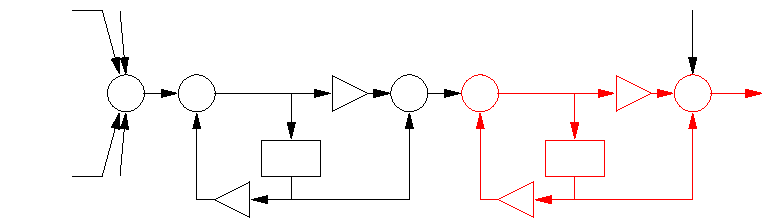
\includegraphics{reverb_diag_des.pdf}%
\end{picture}%
\setlength{\unitlength}{3750sp}%
%
\begingroup\makeatletter\ifx\SetFigFont\undefined%
\gdef\SetFigFont#1#2#3#4#5{%
  \reset@font\fontsize{#1}{#2pt}%
  \fontfamily{#3}\fontseries{#4}\fontshape{#5}%
  \selectfont}%
\fi\endgroup%
\begin{picture}(6927,1683)(-914,-1723)
\put(-135,-409){\makebox(0,0)[lb]{\smash{{\SetFigFont{10}{13.2}{\rmdefault}{\mddefault}{\updefault}{\color[rgb]{0,0,0}-$\alpha$}%
}}}}
\put(-673,-1185){\color[rgb]{0,0,0}$z^{-d}$}%
\put(1876,-1186){\color[rgb]{0,0,0}$z^{-d}$}%
\put(2626,-1186){\color[rgb]{1,0,0}$z^{-d}$}%
\put(3826,-436){\color[rgb]{1,0,0}$\Sigma$}%
\put(1126,-436){\color[rgb]{0,0,0}$\Sigma$}%
\put(526,-436){\color[rgb]{0,0,0}$\Sigma$}%
\put(5126,-1616){\makebox(0,0)[lb]{\smash{{\SetFigFont{10}{13.2}{\rmdefault}{\mddefault}{\updefault}{\color[rgb]{1,0,0}$\alpha$}%
}}}}
\put(5326,-1186){\color[rgb]{1,0,0}$z^{-d}$}%
\put(4426,-436){\color[rgb]{1,0,0}$\Sigma$}%
\put(-899,-286){\color[rgb]{0,0,0}$x[n]$}%
\put(5776,-286){\color[rgb]{1,0,0}$y[n]$}%
\put(1876,-211){\color[rgb]{1,0,0}\textit{Multiply times}}%
\put(1663,-1610){\makebox(0,0)[lb]{\smash{{\SetFigFont{10}{13.2}{\rmdefault}{\mddefault}{\updefault}{\color[rgb]{0,0,0}$\alpha$}%
}}}}
\put(3165,-408){\makebox(0,0)[lb]{\smash{{\SetFigFont{10}{13.2}{\rmdefault}{\mddefault}{\updefault}{\color[rgb]{1,0,0}-$\alpha$}%
}}}}
\end{picture}%
  \caption{The figure shows a block diagram of a \gls{reverb} unit.}
  \label{fig:reverb_block_des}
\end{figure}

From \autoref{fig:reverb_block_des}, the following differential equations can be inferred:

The equation for the delay can be written as:
\begin{equation}
\label{eq:delay_eq}
		y[n] = - \alpha \cdot x[n] + x[n-d] + \alpha \cdot y[n-d]
\end{equation}

The \gls{reverb} unit is more advanced than the delay unit and before the differential equations can be inferred, some calculation is needed. The \gls{reverb} unit calculation are based on a article \citep{natural_sounding_revorb} which explain the design parametric for a \gls{reverb} unit very well. Form \citep{natural_sounding_revorb} the \gls{reverb} time is defined by \autoref{eq:reverb_defined}

\begin{equation}
\label{eq:reverb_defined}
		T = \frac{60}{-20 \cdot log(\alpha)} \cdot \tau
\end{equation}

    \startexplain
\explain{$60$ is the \gls{reverb} attenuation in \si{\decibel}, and the \gls{reverb} time is defined that a given signal is attenuated by 60 \si{\decibel}}{\si{\decibel}}

\explain{$\tau$ is the delay over the sample frequency $\tau = \frac{d}{f_s}$}{\si{\second}}

\explain{$T$ is the resulting \gls{reverb} time}{\si{\second}}

\explain{$-20 \cdot log10(\alpha)$ is the attenuation in the feedback loop for each round}{\si{\decibel}}
    \stopexplain

The gain $\alpha$ is is chosen to be 0.708 like useal \gls{reverb} unit  \citep{natural_sounding_revorb} and the total \gls{reverb} echo density shall at lest be 1000 echo per second. In formula \autoref{eq:reverb_defined_tal_res} it can be obtain that $\tau$ shall be $\frac{1}{20}$ of $T$


\begin{subequations}
\begin{equation}\label{eq:reverb_defined_tal}
       T = \frac{60}{-20 \cdot log(0.7)} \cdot \tau
       \addunit{\si{\second}}
    \end{equation}
\centering
$\Updownarrow$
\begin{equation}\label{eq:reverb_defined_tal_res}
        \tau = \frac{1}{20} T
        \addunit{\si{\second}}
    \end{equation}
 \end{subequations}

\autoref{eq:reverb_defined_tal_res} then shows that the $\tau$ time is \SI{50}{\milli\second} with a total \gls{reverb} time $T$ of \SI{1}{second}. This achieve an echo density of 20 echo per second, but the \gls{reverb} unit require 1000 echo per second \citep{natural_sounding_revorb}. To achieve 1000 echo per second there needs to be multiply delay unit in serial. To calculate the number of needed \gls{reverb} unit a formula is obtained and the $n$ symbolize the number of \gls{reverb} unit in \autoref{eq:reverb_needed} 

\begin{equation}
\label{eq:reverb_needed}
		\frac{1}{\tau} \cdot k^{n-1} \geq  \text{echo density}
		\addunit{\si{\second}}
\end{equation}

    \startexplain
\explain{\textit{echo density} is the number for echo per second}{\si{1}}
\explain{$\tau$ is the delay over the sample frequency $\tau = \frac{d}{f_s}$}{\si{\second}}
\explain{$k$ is the scaling factor between each \gls{reverb} unit, which normally is a factor of tree \citep{natural_sounding_revorb}}{\si{1}}
\explain{$n$ is the required number of \gls{reverb} unit}{\si{1}}
    \stopexplain

The \autoref{eq:reverb_needed}  can be rewritten to \autoref{eq:reverb_defined_tal_mellem}


\begin{subequations}
\begin{equation}\label{eq:reverb_needed_solve}
		\frac{1}{\SI{50}{\milli\second}} \cdot 3^{n-1} \geq  1000
		\addunit{\si{1}}
    \end{equation}
\centering
$\Updownarrow$
\begin{equation}\label{eq:reverb_defined_tal_mellem}
        n \geq  \frac{ln(3)+ln{1000 \cdot T}}{ln(3)}
        \addunit{\si{1}}
    \end{equation}
    $\Updownarrow$
\begin{equation}\label{eq:reverb_defined_tal_res}
        n \geq  4.56
        \addunit{\si{1}}
    \end{equation}
 \end{subequations}

Since the number of the \gls{reverb} unit only can be integer, the needed numbers of \gls{reverb} unit is 5.

\newpage

\begin{figure} [htbp]
 \centering
\begin{picture}(0,0)%
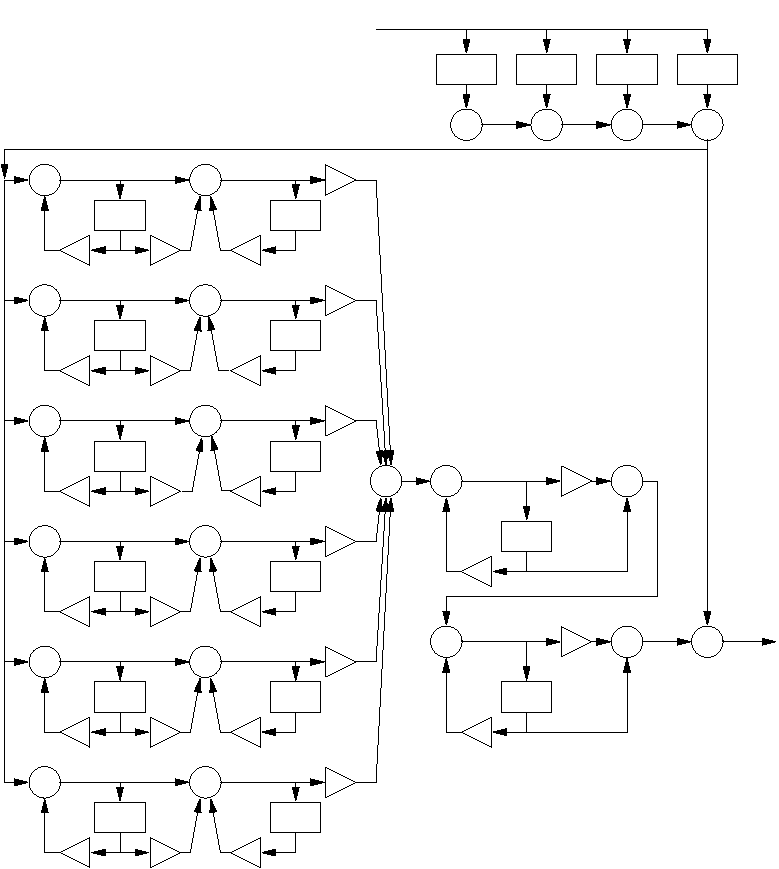
\includegraphics{reverb_serial_des.pdf}%
\end{picture}%
\setlength{\unitlength}{3937sp}%
%
\begingroup\makeatletter\ifx\SetFigFont\undefined%
\gdef\SetFigFont#1#2#3#4#5{%
  \reset@font\fontsize{#1}{#2pt}%
  \fontfamily{#3}\fontseries{#4}\fontshape{#5}%
  \selectfont}%
\fi\endgroup%
\begin{picture}(5319,4317)(436,-4393)
\put(2881,-3121){w5[n]}%
\put(4771,-1276){a}%
\put(4951,-916){$z^{-d}$}%
\put(3151,-916){$z^{-d}$}%
\put(3736,-376){-a}%
\put(4231,-421){$\Sigma$}%
\put(2431,-916){$z^{-d}$}%
\put(1216,-376){-a}%
\put(631,-916){$z^{-d}$}%
\put(2251,-1276){a}%
\put(1711,-421){$\Sigma$}%
\put(1216,-1816){-a}%
\put(631,-2356){$z^{-d}$}%
\put(1711,-1861){$\Sigma$}%
\put(3736,-1816){-a}%
\put(4771,-2716){a}%
\put(4231,-1861){$\Sigma$}%
\put(3151,-2356){$z^{-d}$}%
\put(2431,-2356){$z^{-d}$}%
\put(2251,-2716){a}%
\put(1216,-3256){-a}%
\put(586,-3796){$z^{-d}$}%
\put(2251,-4156){a}%
\put(2431,-3796){$z^{-d}$}%
\put(4951,-2356){$z^{-d}$}%
\put(5356,-1681){w4[n]}%
\put(2881,-1681){w3[n]}%
\put(2881,-241){w1[n]}%
\put(5356,-241){w2[n]}%
\put(451,-241){x[n]}%
\put(1711,-3301){$\Sigma$}%
\put(4231,-3301){$\Sigma$}%
\put(5446,-3121){y[n]}%
\end{picture}%

  \caption{The figure shows a block diagram of a \gls{reverb} unit.}
  \label{fig:reverb_block_des}
\end{figure}




%
%The equation for the \gls{reverb} can be written as:
%
%\begin{equation}
%\label{eq:reverb_eq}
%		y[n] = - \alpha \cdot x[n] + x[n-d] + \alpha \cdot y[n-d]
%\end{equation}

%The index $i$ represents the number of delays that are being implemented in the chorus effect which is also the chorus size. Index $n$ represents the number of samples that are being modulated. \\
%If the implementation is done using a time varying delay, equations \ref{flang_eq} and \ref{chor_eq} can be re-written as:
%
%\begin{equation}
%\label{flang_eq2}
%y[n] = x[n] + x[n- d_{1}[n]] \cdot g_{1}  
%\end{equation}
%
%\begin{equation}
%\label{chor_eq2}
%y[n] = x[n] + \sum_{j=1}^{i}  (x[n- d_{j}[n]] \cdot g_{j})
%\end{equation}
%
%The delay value has to be a periodic function that is varying in a user-defined range. 
%
%\subsection{Matlab Simulation}
%
%A delay can be done in different ways digitally. One way is to use a ring buffer also known as circular buffer. \\
%The idea of this data structure is that it takes values and only outputs them when it gets full, and overwrites the oldest after outputting it. It is a kind of a FIFO queue structure but where the start and the overwriting can start at any index. \\
%This means that the size of the buffer depends on the delay.  The buffer size must then be always up-to-date with the new delay value. \\ 
%The value of the delay is determined by a periodic function as said before, different waveforms can be used as said in \autoref{chor_flang}. A common periodic function that can be used is the sine. Since it varies between 0 and 1, it can be then multiplied with the user-defined range. 
%The delay can then be written as:
%
%\begin{equation}
%	d[n]= A \cdot sin(2\pi f_{l} n)
%\end{equation}
%
%$A$ is the value of the user-defined range which is also the depth. $f_{l}$ is the frequency of the LFO. 
%
%The Matlab code for the flanger effect is:
%
%\begin{lstlisting}[language=Matlab, caption= Matlab code for flanger effect]
%
%%Flanger Effect
%%Group 641
%
%%insert your input in this table
%input = [1 2 3 4 5 6 7 8 9 10]
%
%fs = 1;  %LFO Frequency
%sample_no = length(input) %Length of the input
%g = 0.4; %Gain
%after_delay = (1:1:sample_no); 
%before_delay = (1:1:sample_no);
%output = (1:1:sample_no);
%
%for n = 1:1:sample_no
%	delay = 3 * cos((2*pi*fs)/n);  %Calculate time varying delay
%	buffer = zeros(1,abs(round(delay)));
%
%	for i = 1:1:sample_no %loop for an output with one delay value
%		buffer = [buffer(2:end) input(i)];
%		after_delay(i) = buffer(1) * g;
%		before_delay(i) = input(i); 
%		output(i) = after_delay(i) + before_delay(i);
%	end
%	output
%end
%
%plot(output)
%hold on
%grid
%plot(before_delay)
%
%\end{lstlisting}
%
%
%
%
%
